\documentclass[uplatex,dvipdfmx]{jsarticle}
\和暦
\usepackage[top=25truemm,bottom=25truemm,left=25truemm,right=25truemm]{geometry}
\usepackage[dvipdfmx]{graphicx}
\usepackage{color}
\usepackage{listings}
\usepackage[bookmarks=true,bookmarksnumbered=true,bookmarkstype=toc]{hyperref}
\usepackage{pxjahyper}
\hypersetup{pdftitle={lda.pyのtest setsでの学習について},pdfauthor={木村 健},
  pdfkeywords={upTeX,upLaTeX,LDA,NIPS,ja.text8,20newsgroups}}
\definecolor{dkgreen}{rgb}{0,0.6,0}
\definecolor{gray}{rgb}{0.5,0.5,0.5}
\definecolor{mauve}{rgb}{0.58,0,0.82}

\lstset{frame=tb,
  language=Python,
  aboveskip=3mm,
  belowskip=3mm,
  showstringspaces=false,
  columns=flexible,
  basicstyle={\small\ttfamily},
  numbers=none,
  numberstyle=\tiny\color{gray},
  keywordstyle=\color{blue},
  commentstyle=\color{dkgreen},
  stringstyle=\color{mauve},
  breaklines=true,
  breakatwhitespace=true,
  tabsize=3
}
\begin{document}

\title{\huge lda.pyのtest setsでの学習について}
\author{木村 健}
\date{\today}
\maketitle


\section{このドキュメントについて}
本ドキュメントは持橋先生が作成されたlda.pyについて、
三種類のテストセットで実際どのようにトピック付けがなされるかを
報告するものである。

\section{LDAのタスクと入力パラメータ}
LDA\cite{blei}はドキュメント群(ここでは簡単のため英語とする)
の各単語について潜在的トピックを推定する技法である。
いくつのトピックに分けるかは最初に指定する。常に同じ順序でトピックが抽出されると限らない。
unsupervised learningである(教師値を用いない)。

LDAの開始に先立って次のパラメータが必要となる(LDA.pyのindex.htmlより引用加筆)
Gibbs samplingという技法を利用していることを付け加えておく。

\begin{itemize}
\item K: topics: number of topics in LDA
\item N: iters: number of Gibbs iterations
\item $\alpha$: Dirichlet hyperparameter on topics
\item $\beta$: Dirichlet hyperparameter on words
\end{itemize}

Kがトピック数で、はじめに与える。例えば$K=10$とする。
Nはイテレーションの回数でこれを大きくするほどperplexityが改善(小さくなる)するが
ある程度まで行くとあまり動かなくなる。

\section{NIPS}
Abstract: This data set contains the distribution of words in the full text of the NIPS conference papers published from 1987 to 2015.

Data Set Characteristics:  

Text

Number of Instances:

11463

Area:

Computer

Attribute Characteristics:

Integer

Number of Attributes:

5812

Date Donated

2016-11-23

Associated Tasks:

Clustering

Missing Values?

N/A

Number of Web Hits:

28333



Data Set Information:

The dataset is in the form of a 11463 x 5812 matrix of word counts, containing 11463 words and 5811 NIPS conference papers (the first column contains the list of words). Each column contains the number of times each word appears in the corresponding document. The names of the columns give information about each document.


NIPSは学会であるNIPSに投稿された論文について、documents x words のCSV(密行列)
を提供するもので、低頻度単語のomitや正規化を行ったデータセットである。
\begin{figure}[t]
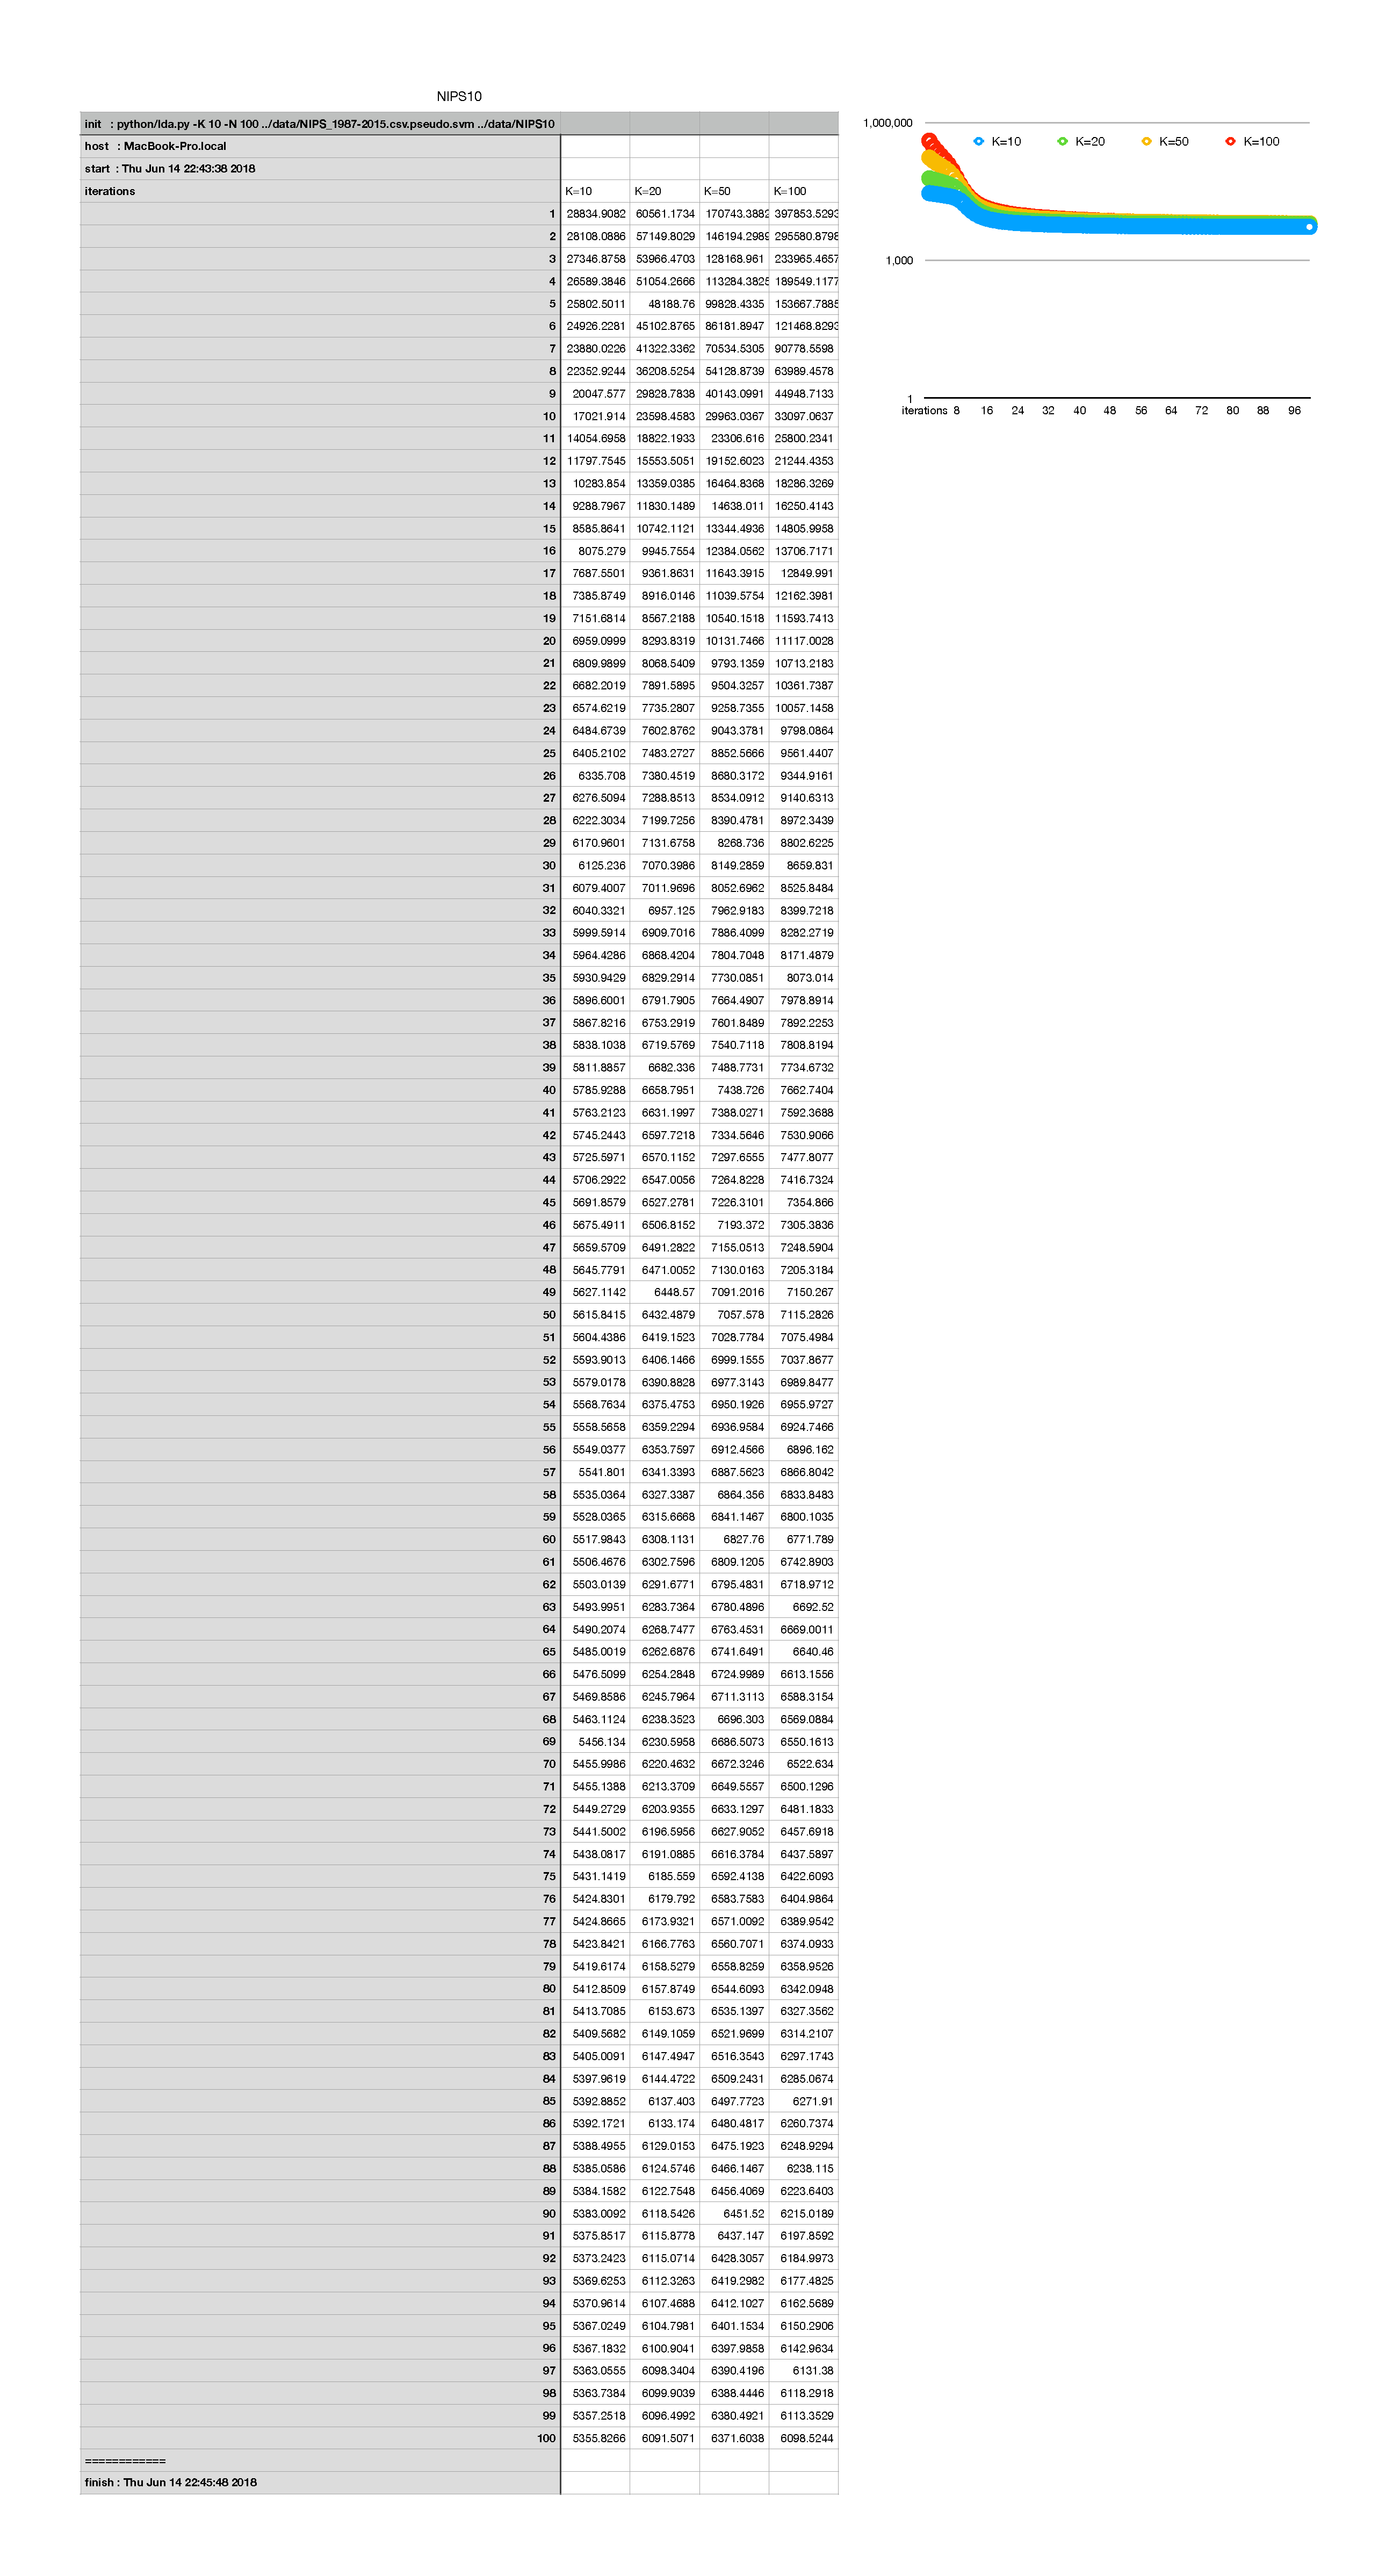
\includegraphics[width=13cm,pagebox=cropbox]{NIPS.pdf}
\caption{NIPS}
\end{figure}

\begin{figure}[ht]
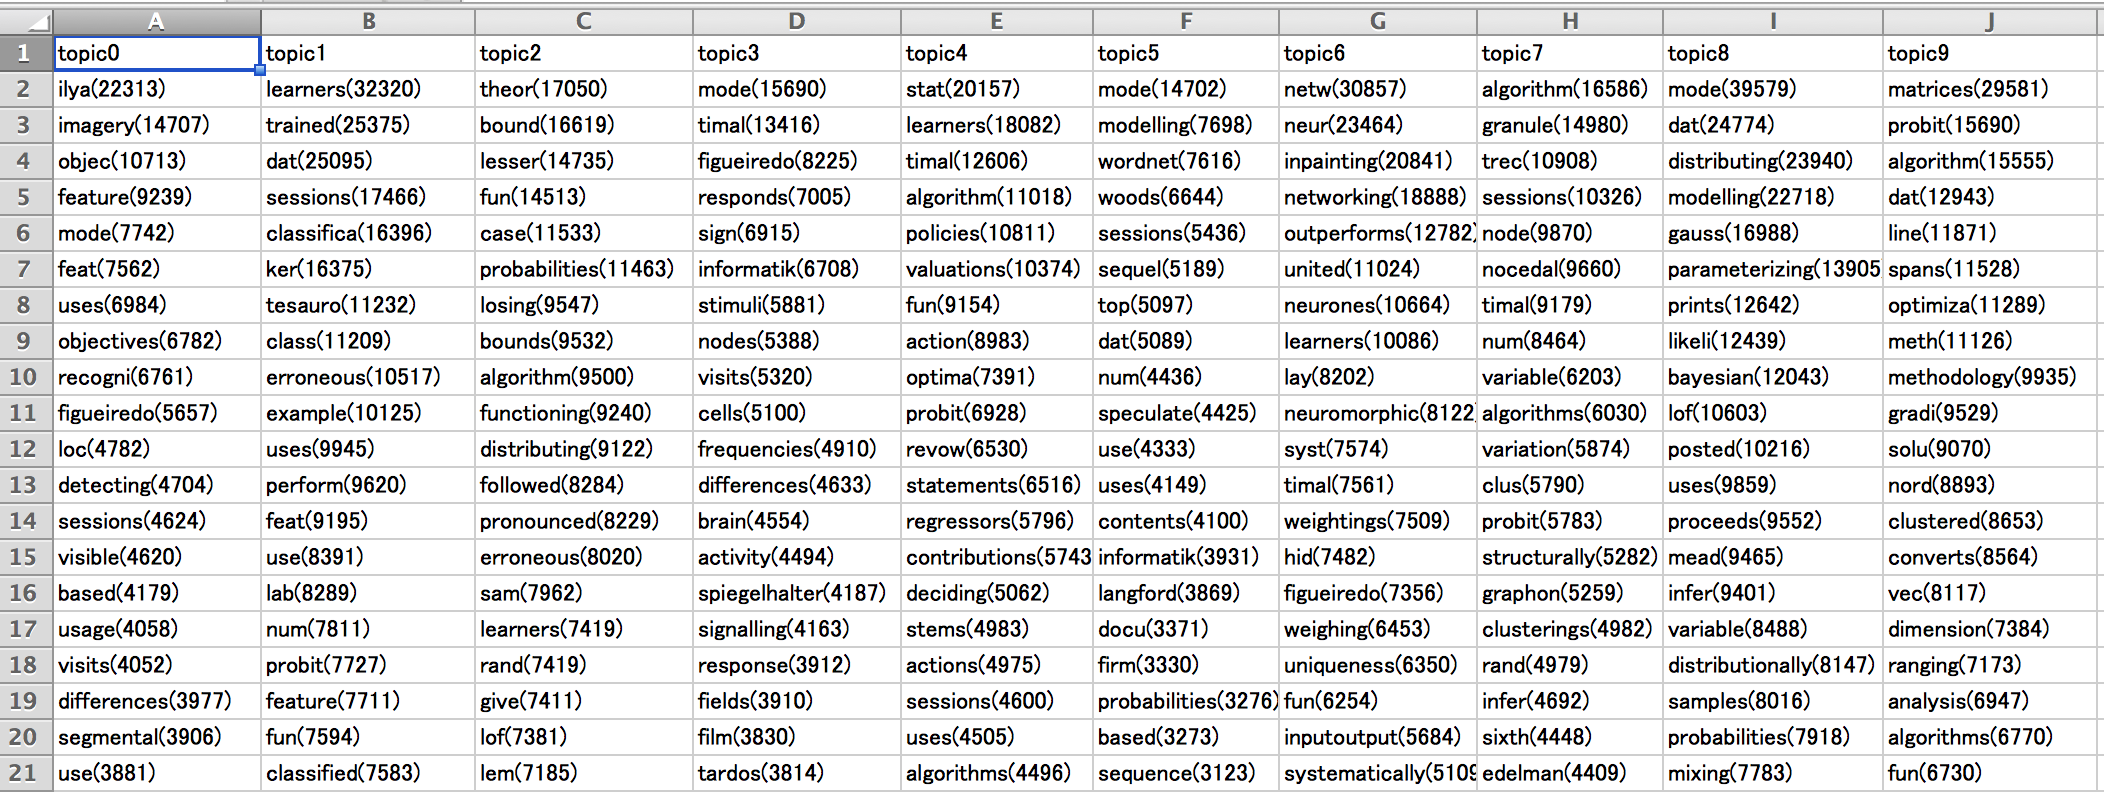
\includegraphics[width=16cm]{NIPS10.png}
\caption{分類結果(NIPS)}
\end{figure}

\section{The 20 Newsgroups data set}

The 20 Newsgroups data set is a collection of approximately 20,000 newsgroup documents, partitioned (nearly) evenly across 20 different newsgroups. To the best of my knowledge, it was originally collected by Ken Lang, probably for his Newsweeder: Learning to filter netnews paper, though he does not explicitly mention this collection. The 20 newsgroups collection has become a popular data set for experiments in text applications of machine learning techniques, such as text classification and text clustering.

Organization
The data is organized into 20 different newsgroups, each corresponding to a different topic. Some of the newsgroups are very closely related to each other (e.g. comp.sys.ibm.pc.hardware / comp.sys.mac.hardware), while others are highly unrelated (e.g misc.forsale / soc.religion.christian). Here is a list of the 20 newsgroups, partitioned (more or less) according to subject matter:
\begin{itemize}
\item comp.graphics
\item comp.os.ms-windows.misc
\item comp.sys.ibm.pc.hardware
\item comp.sys.mac.hardware
\item comp.windows.x	rec.autos
\item rec.motorcycles
\item rec.sport.baseball
\item rec.sport.hockey	sci.crypt
\item sci.electronics
\item sci.med
\item sci.space
\item misc.forsale
\item talk.politics.misc
\item talk.politics.guns
\item talk.politics.mideast
\item talk.religion.misc
\item alt.atheism
\item soc.religion.christian
\end{itemize}

Data
The data available here are in .tar.gz bundles. You will need tar and gunzip to open them. Each subdirectory in the bundle represents a newsgroup; each file in a subdirectory is the text of some newsgroup document that was posted to that newsgroup.

Below are three versions of the data set. The first ("19997") is the original, unmodified version. The second ("bydate") is sorted by date into training(60\%) and test(40\%) sets, does not include cross-posts (duplicates) and does not include newsgroup-identifying headers (Xref, Newsgroups, Path, Followup-To, Date). The third ("18828") does not include cross-posts and includes only the "From" and "Subject" headers.

20news-19997.tar.gz - Original 20 Newsgroups data set
20news-bydate.tar.gz - 20 Newsgroups sorted by date; duplicates and some headers removed (18846 documents)
20news-18828.tar.gz - 20 Newsgroups; duplicates removed, only "From" and "Subject" headers (18828 documents)
I recommend the "bydate" version since cross-experiment comparison is easier (no randomness in train/test set selection), newsgroup-identifying information has been removed and it's more realistic because the train and test sets are separated in time.

昔懐かしいNetNewsの記事を集めたコーパス。bydateを使用。30頻度以下の単語のomitと正規化を実施。
プログラムを作りlda.pyに入力できる形に編集。


\begin{figure}[t]
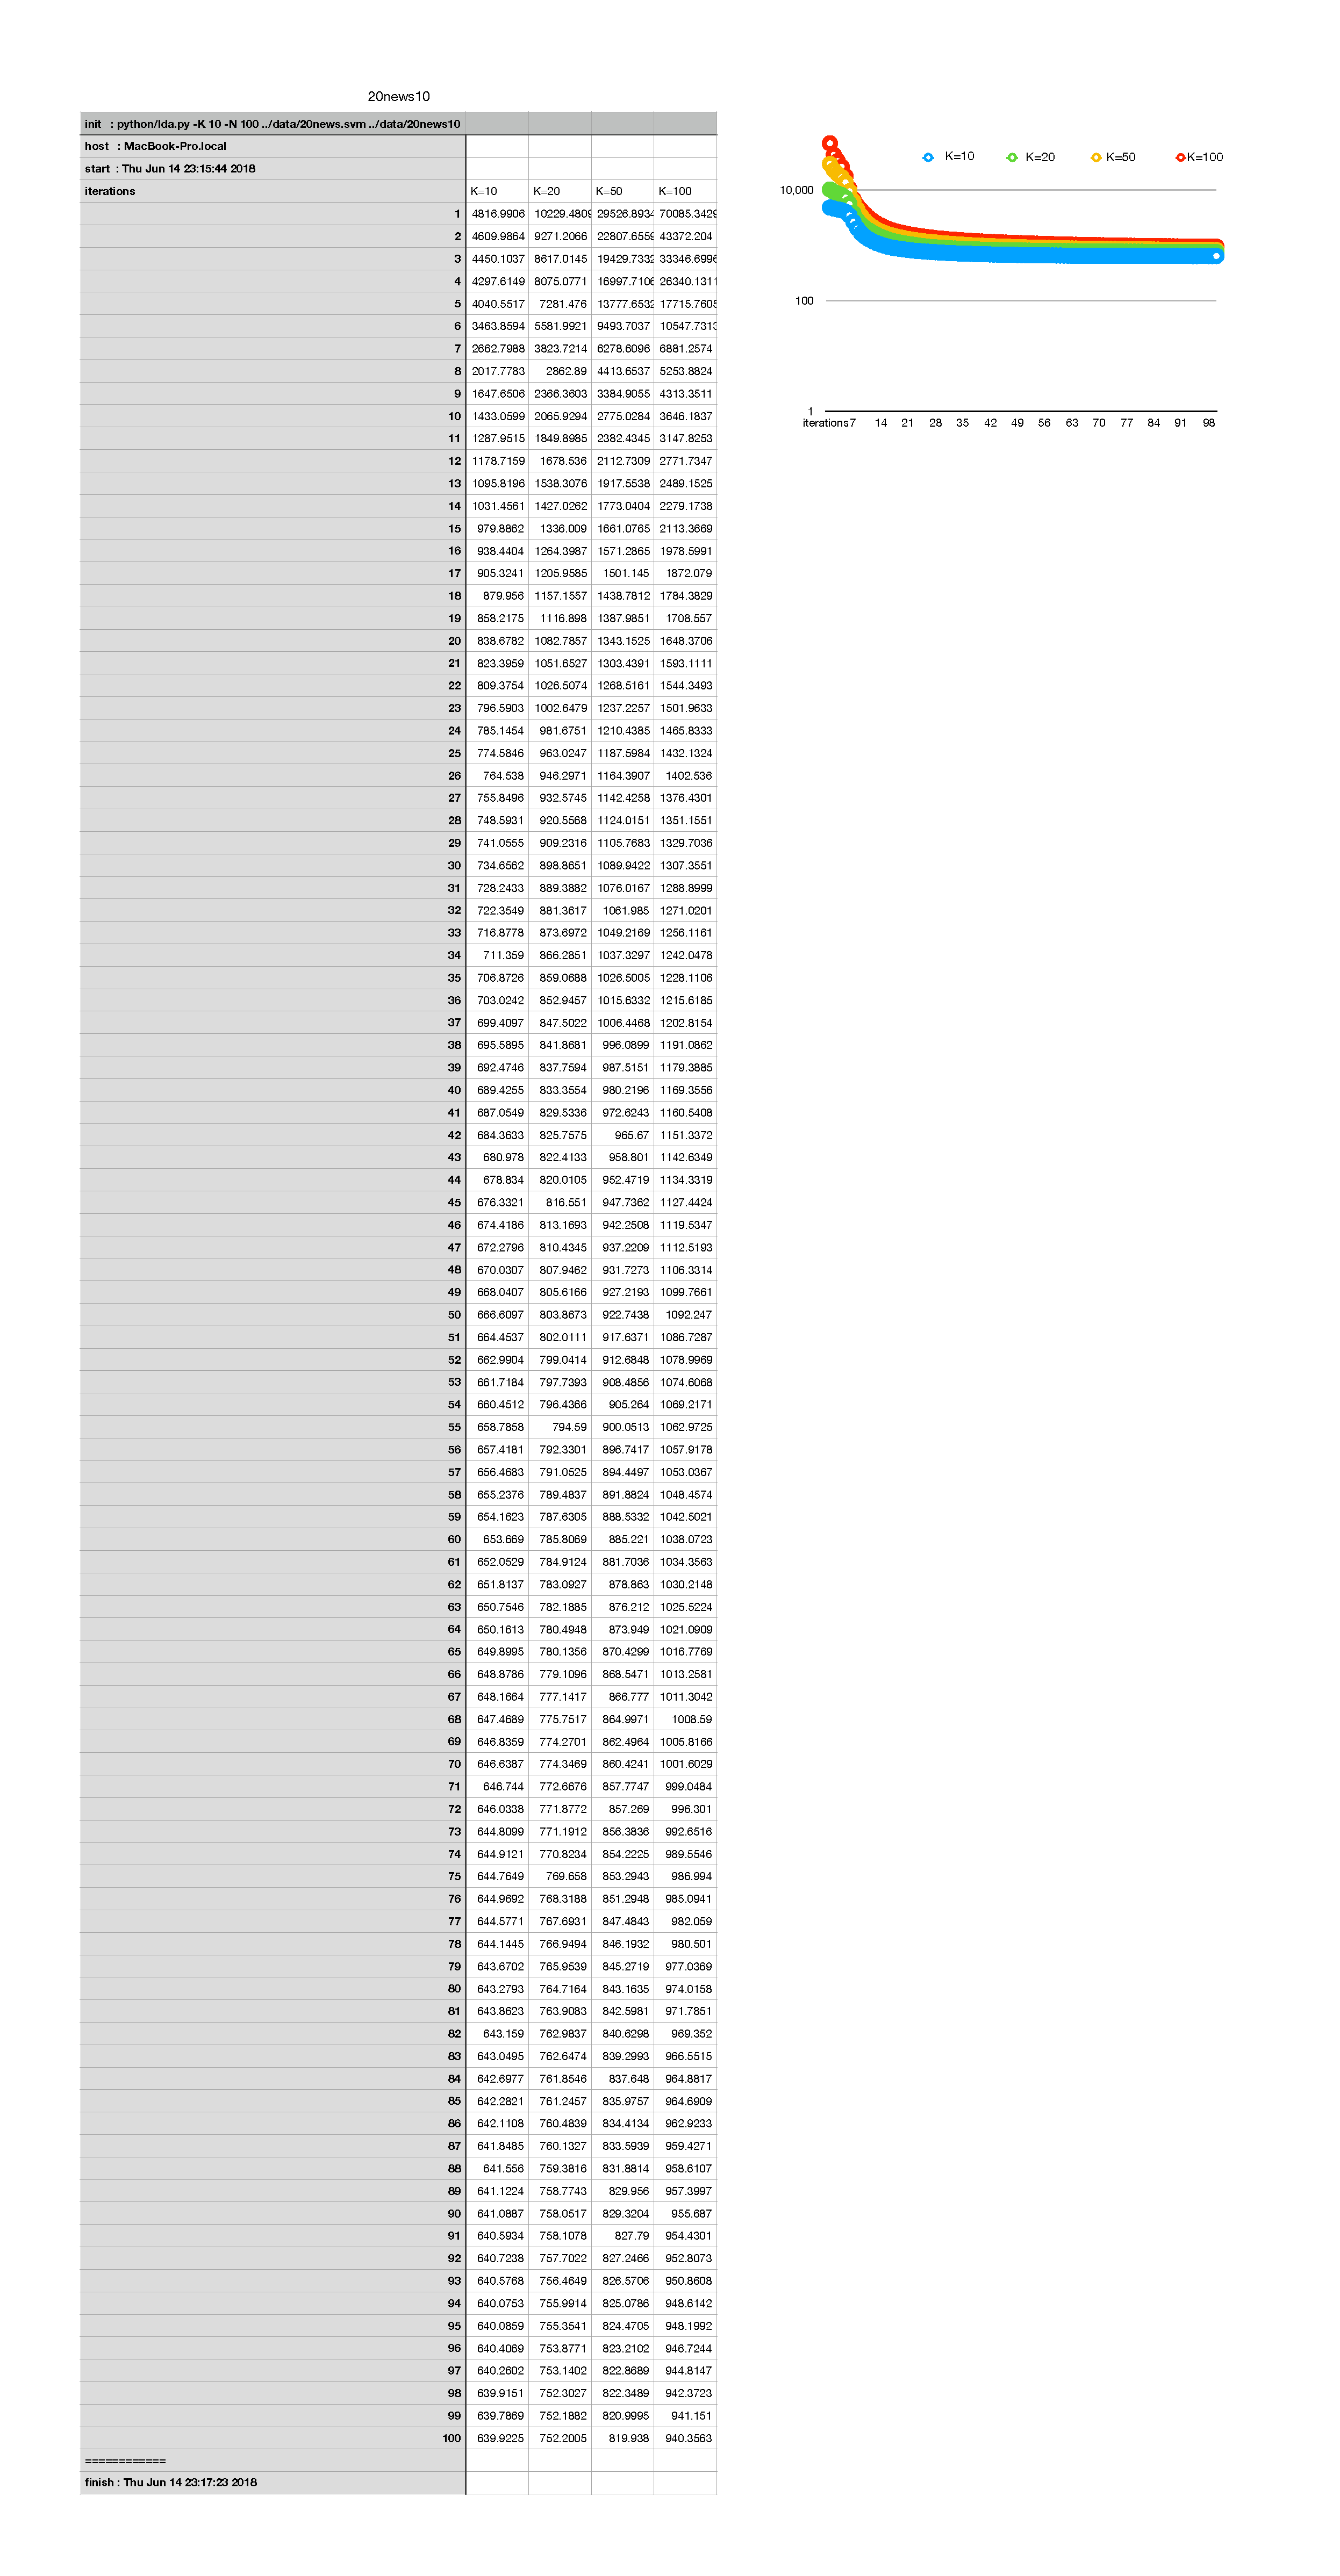
\includegraphics[width=13cm,pagebox=cropbox]{20news.pdf}
\caption{20newsgroups}
\end{figure}

\begin{figure}[ht]
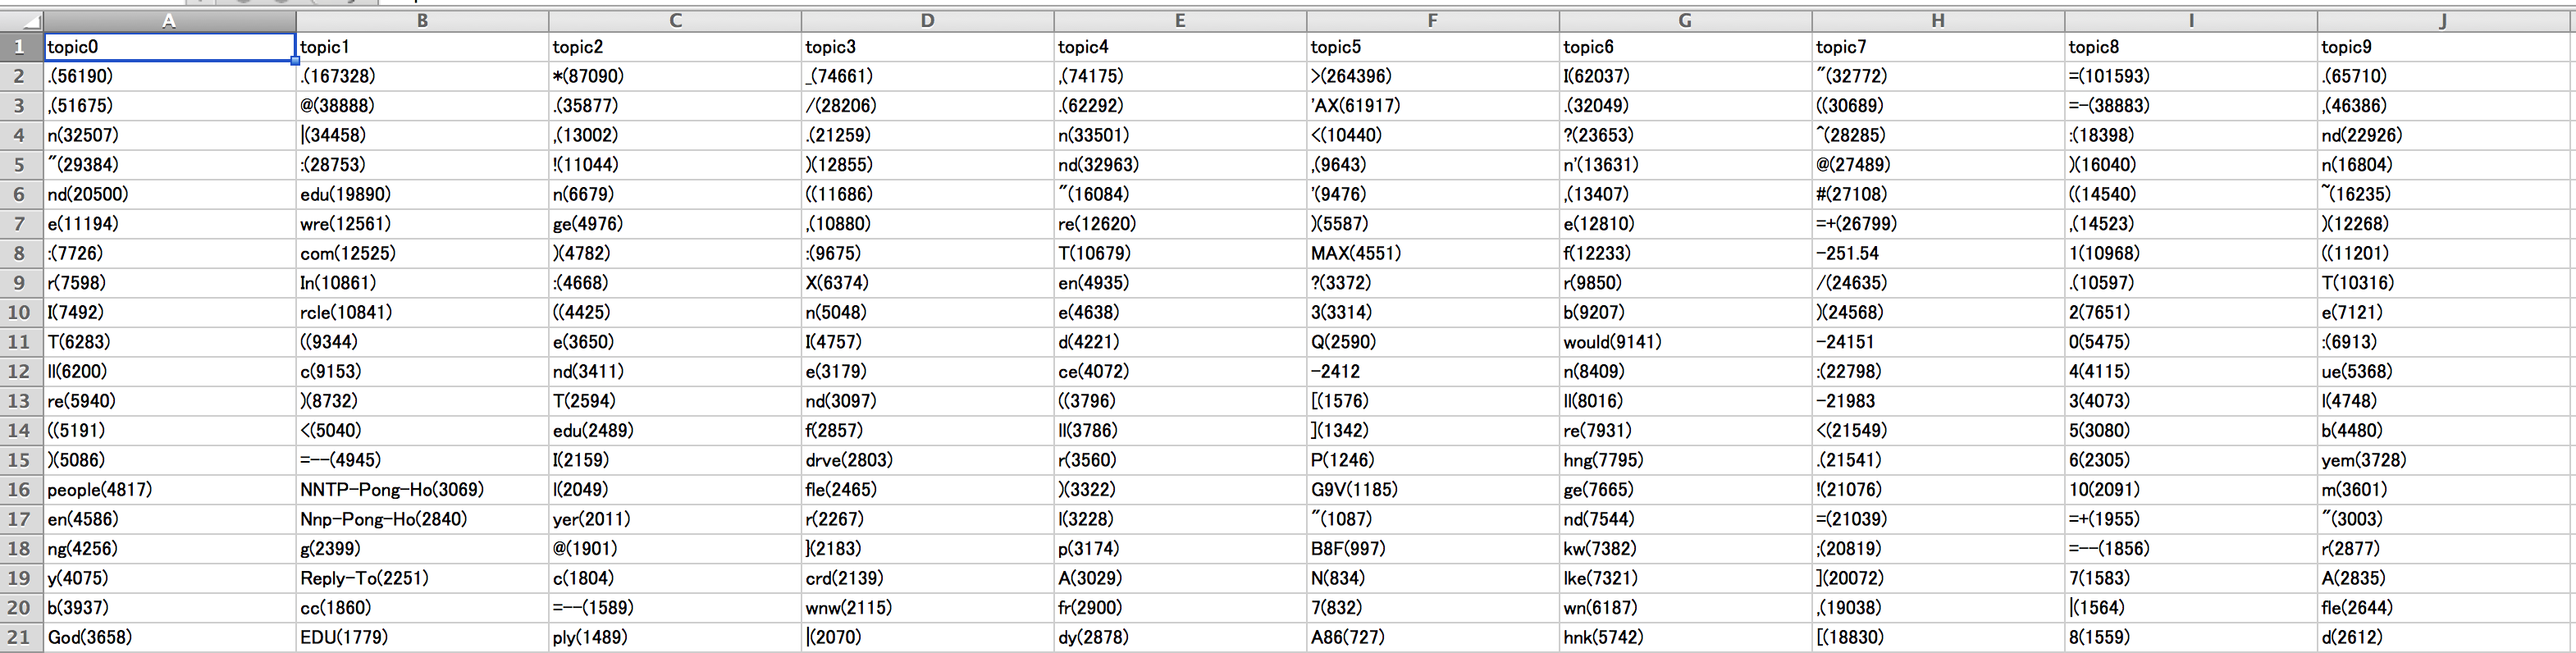
\includegraphics[width=16cm]{20news10.png}
\caption{分類結果(20news)}
\end{figure}

\section{ja.text8}
ja.wikipedia.orgのデータを集め、100MBでcropした日本語コーパス。
ただし、元のコーパスは全て一行に入れられており、ドキュメントごとになってなかったので、
repoをforkして新しいスクリプトを起草。元データが古くwikipediaサイトにも
もうなかったので、比較的新しい(2018/06/01)データでコーパスを再編成した。
30頻度以下の単語のomitをしている。コーパス自体は分かち書き(スペース区切り)が
なされており、一行1ドキュメントである。

original ja.text8 is a small (100MB) text corpus from the web (japanese wikipedia). it modified by kimrin for one line per one article format.

You can download ja.text8 corpus from the following link(original corpus):

this repository contains ja.text8.20180601.100MB that is body of the new corpus.

Requirements
Python 3.x
MeCab

License
CC-BY-SA


\begin{figure}[htb]
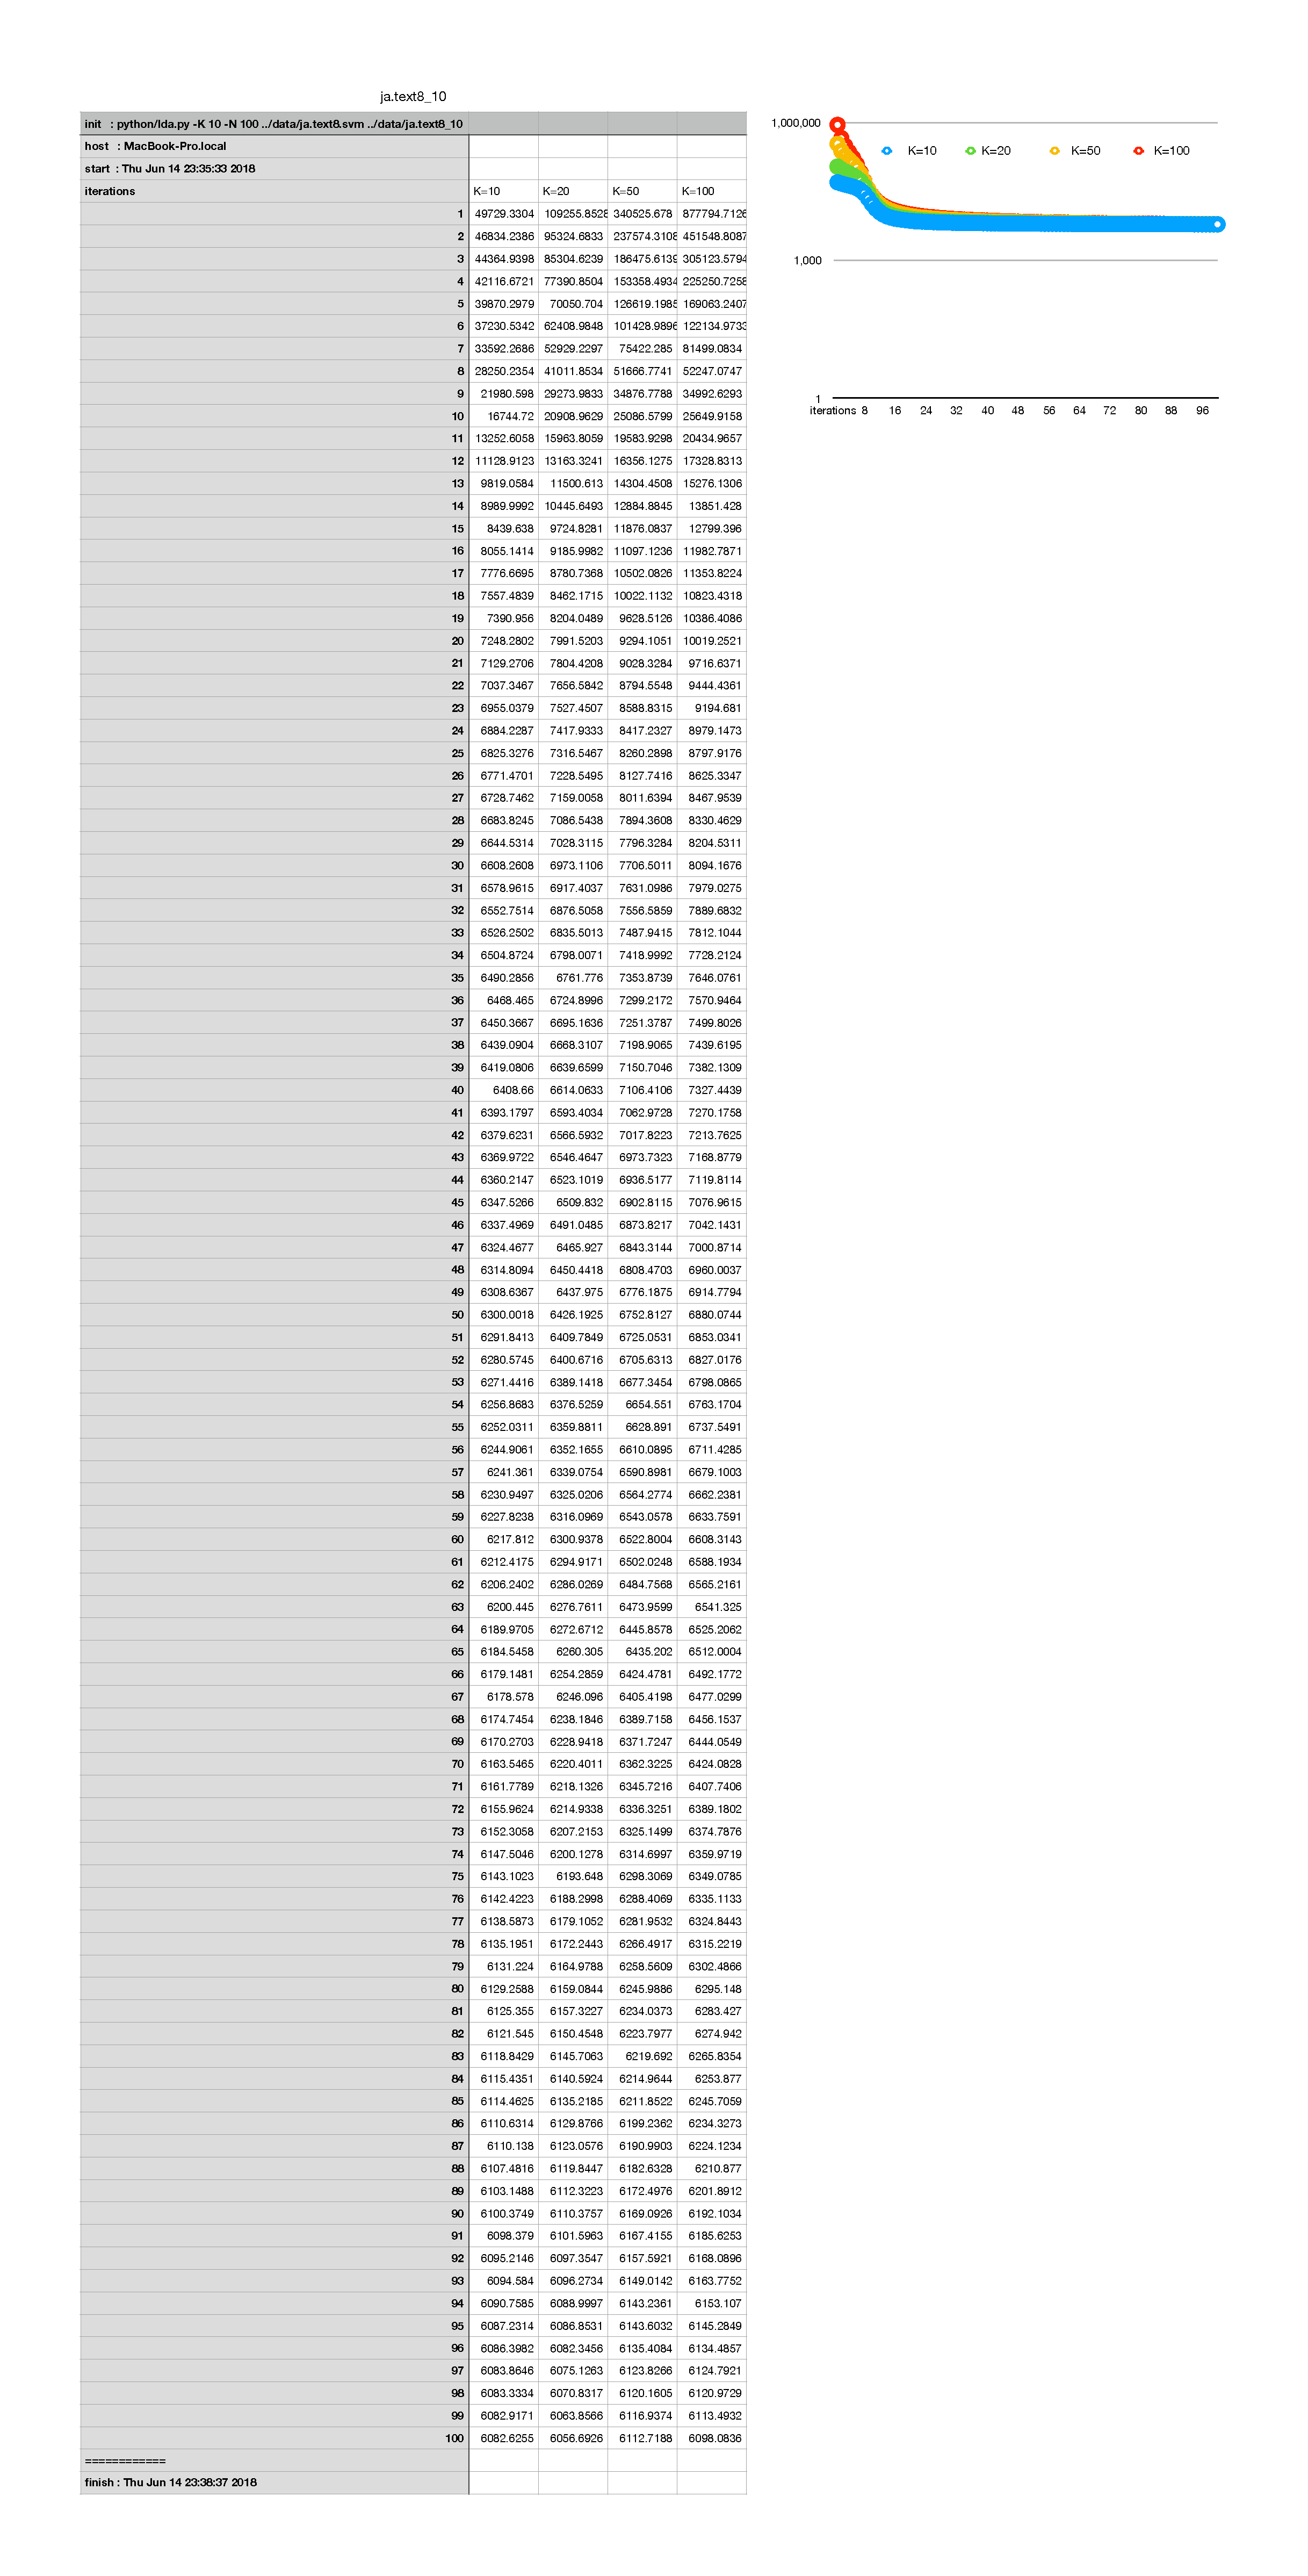
\includegraphics[width=13cm,pagebox=cropbox]{jatext8.pdf}
\caption{ja.text8}
\end{figure}

\begin{figure}[ht]
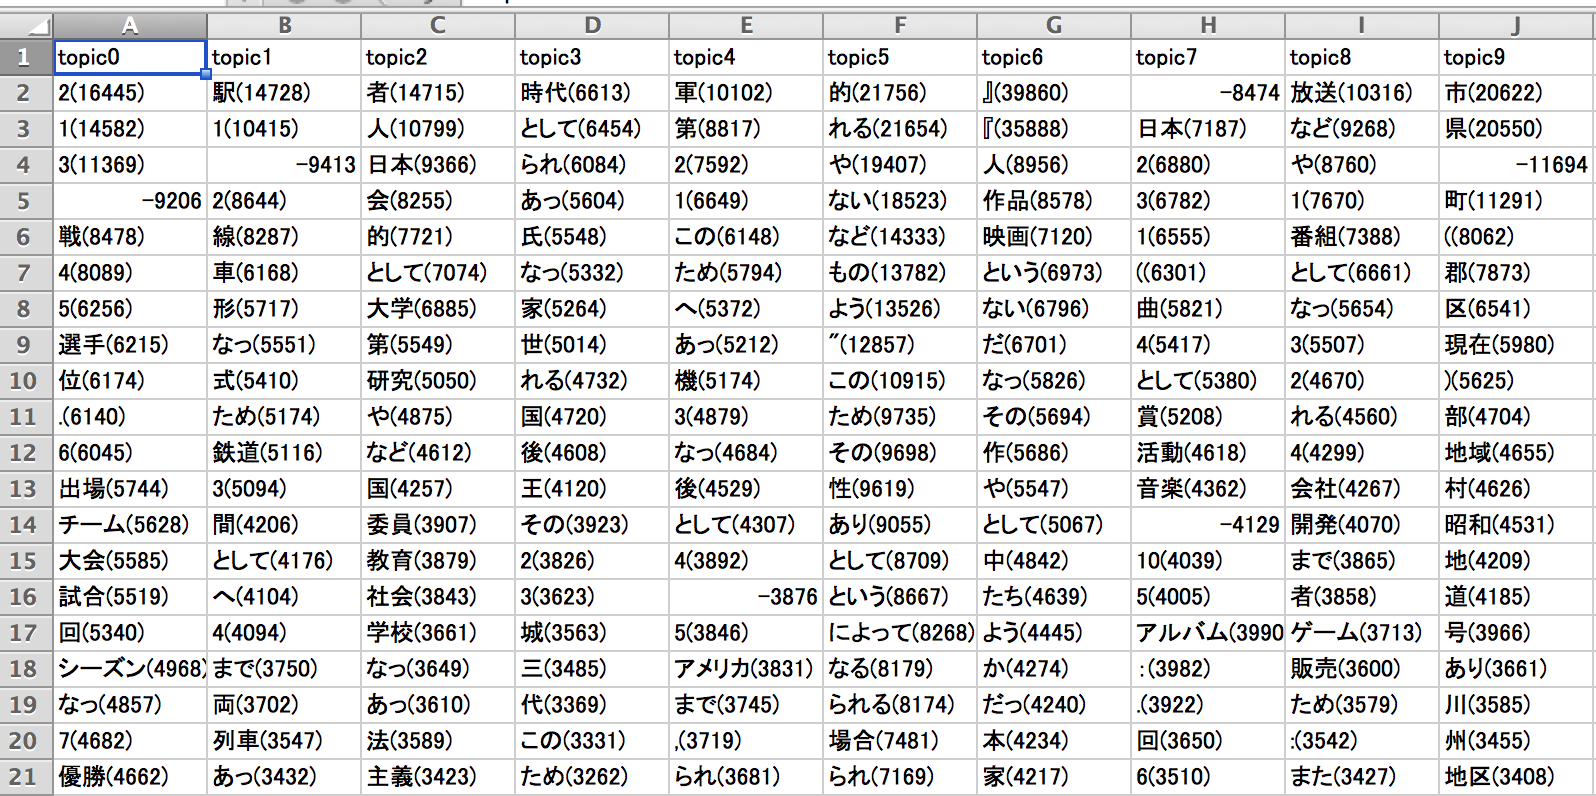
\includegraphics[width=16cm]{jatext810.png}
\caption{分類結果(ja.text8)}
\end{figure}

\section{hyper parameter $\alpha$}
ハイパーパラメータ$\alpha$を変化させてperplexityの変化を見た。
コーパスはja.text8である。

\begin{figure}[htb]
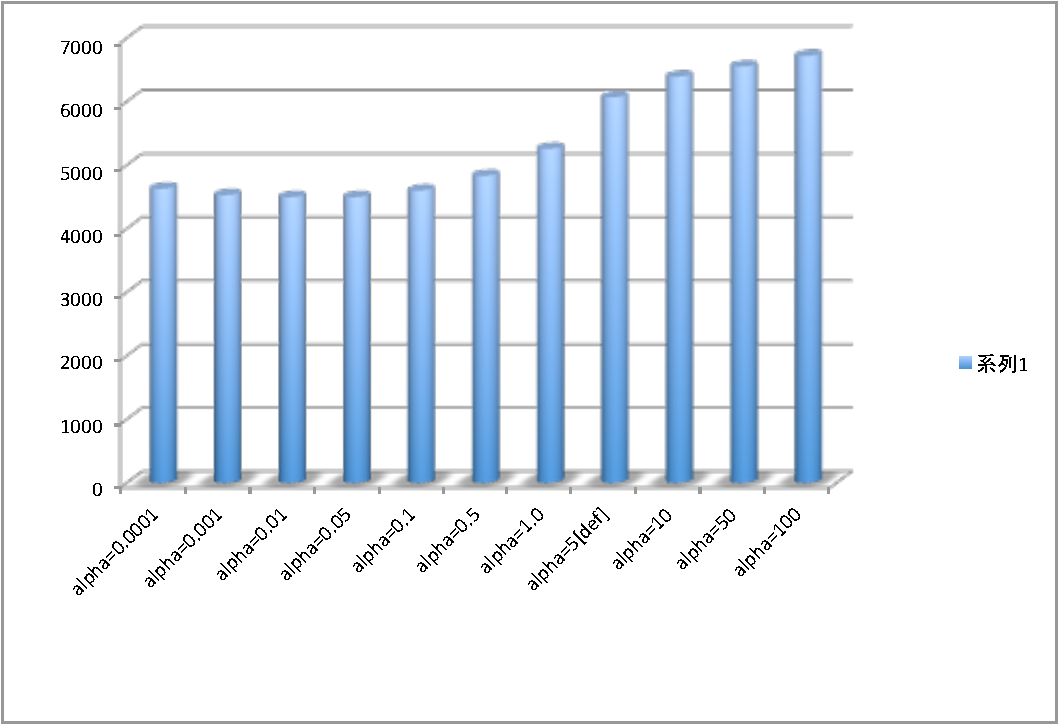
\includegraphics[width=16cm,pagebox=cropbox]{jatext8alpha.pdf}
\caption{alphaを変化させた時のperplexityの変化}
\end{figure}

意外とデフォルトの$50/K$が最良ではないことがわかった。

\section{hyper parameter $\beta$}
ハイパーパラメータ$\beta$を変化させてperplexityの変化を見た。
コーパスはja.text8である。

\begin{figure}[htb]
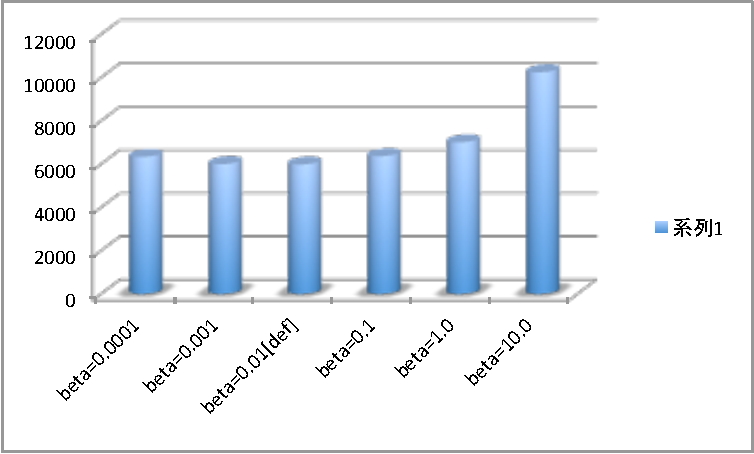
\includegraphics[width=16cm,pagebox=cropbox]{jatext8beta.pdf}
\caption{betaを変化させた時のperplexityの変化}
\end{figure}

こちらは意外と変化は少なかった。$\beta=0.01$が最良でいいと思われる。

\section{後処理の有無によるperplexityの変化}
コーパスは20newsgroupsである。このコーパスは英語かつ平文から
データを作っている関係で、前処理(ストップワードの除去)により
perplexityに変化が出るか測定した。

\begin{figure}[htb]
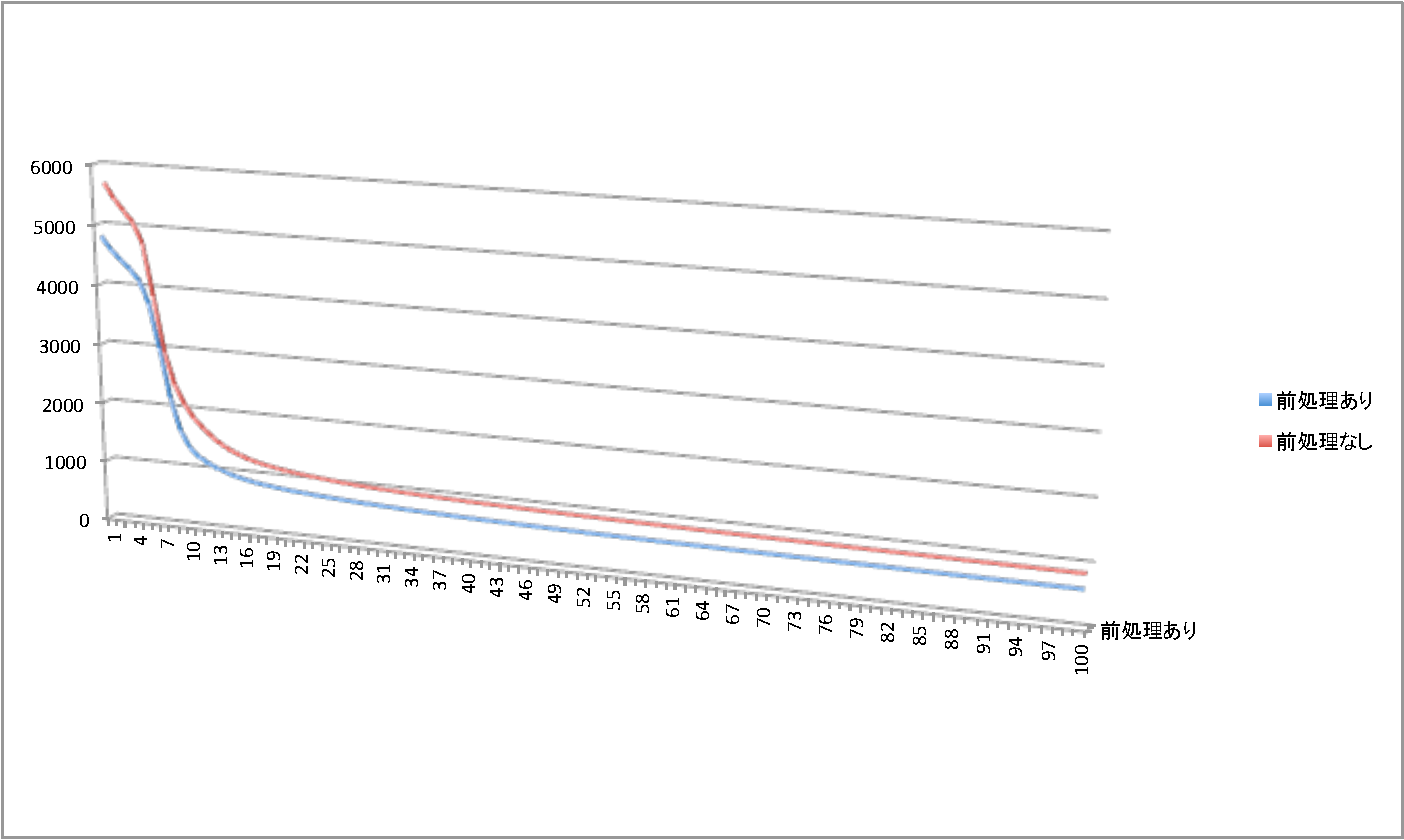
\includegraphics[width=16cm,pagebox=cropbox]{20newspre.pdf}
\caption{前処理を変化させた時のperplexityの変化}
\end{figure}

\section{木村改善案と元のlda.pyの比較}

結論:ほとんど一緒で、topicsのrandomnessを考えるとほぼ誤差。

\begin{figure}[htb]
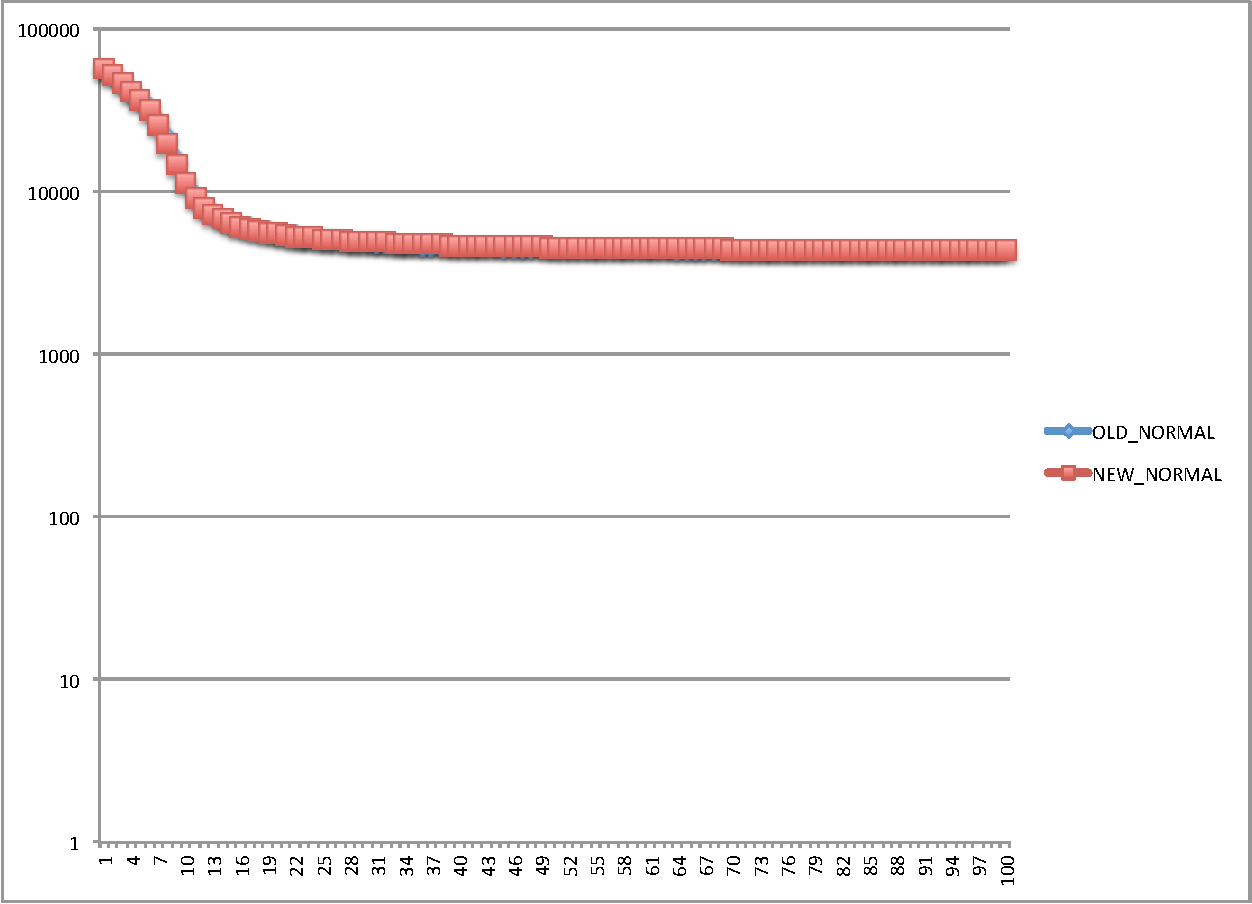
\includegraphics[width=16cm,pagebox=cropbox]{oldandnewnoncool.pdf}
\caption{木村改善案と従来のlda.py}
\end{figure}

\section{coolcutter.pyによる素性除去}
素性数やdfのclampを行うツールで前処理した結果である。

\begin{figure}[htb]
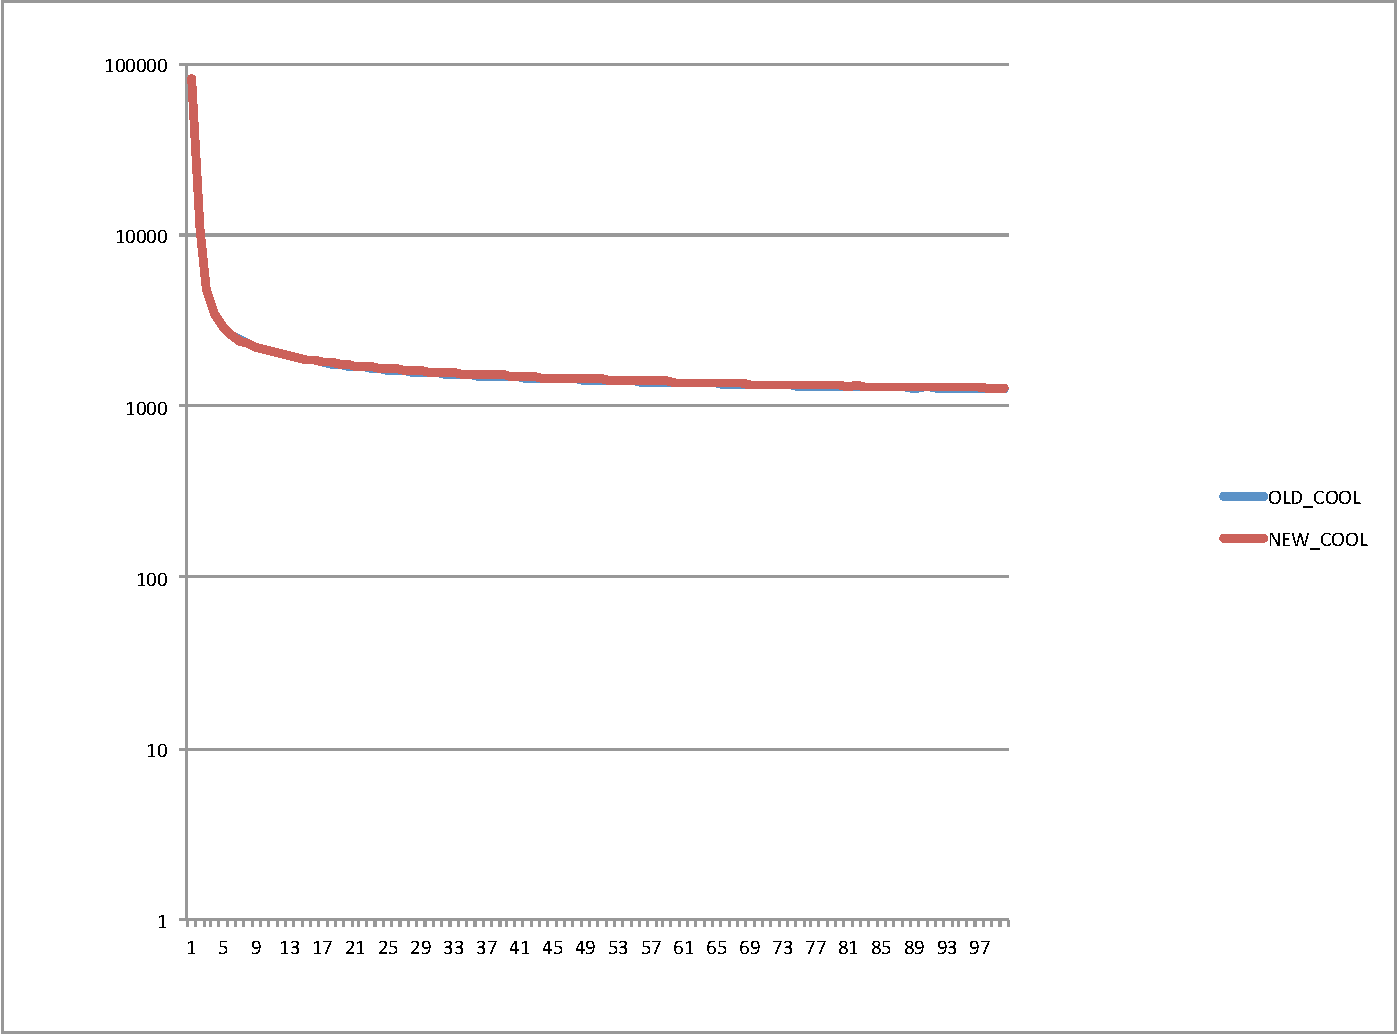
\includegraphics[width=16cm,pagebox=cropbox]{oldandnewcool.pdf}
\caption{木村改善案と従来のlda.py(coolcutter.py済み)}
\end{figure}

こちらは$perplexity=1200$ぐらいで落ち着いた。

\section{木村改善案と元のlda.pyの比較(topics)}
分類結果について図示する(元=OLD, 木村=NEW、COOLのついているものはcoolcutter.py済み)

\begin{figure}[htb]
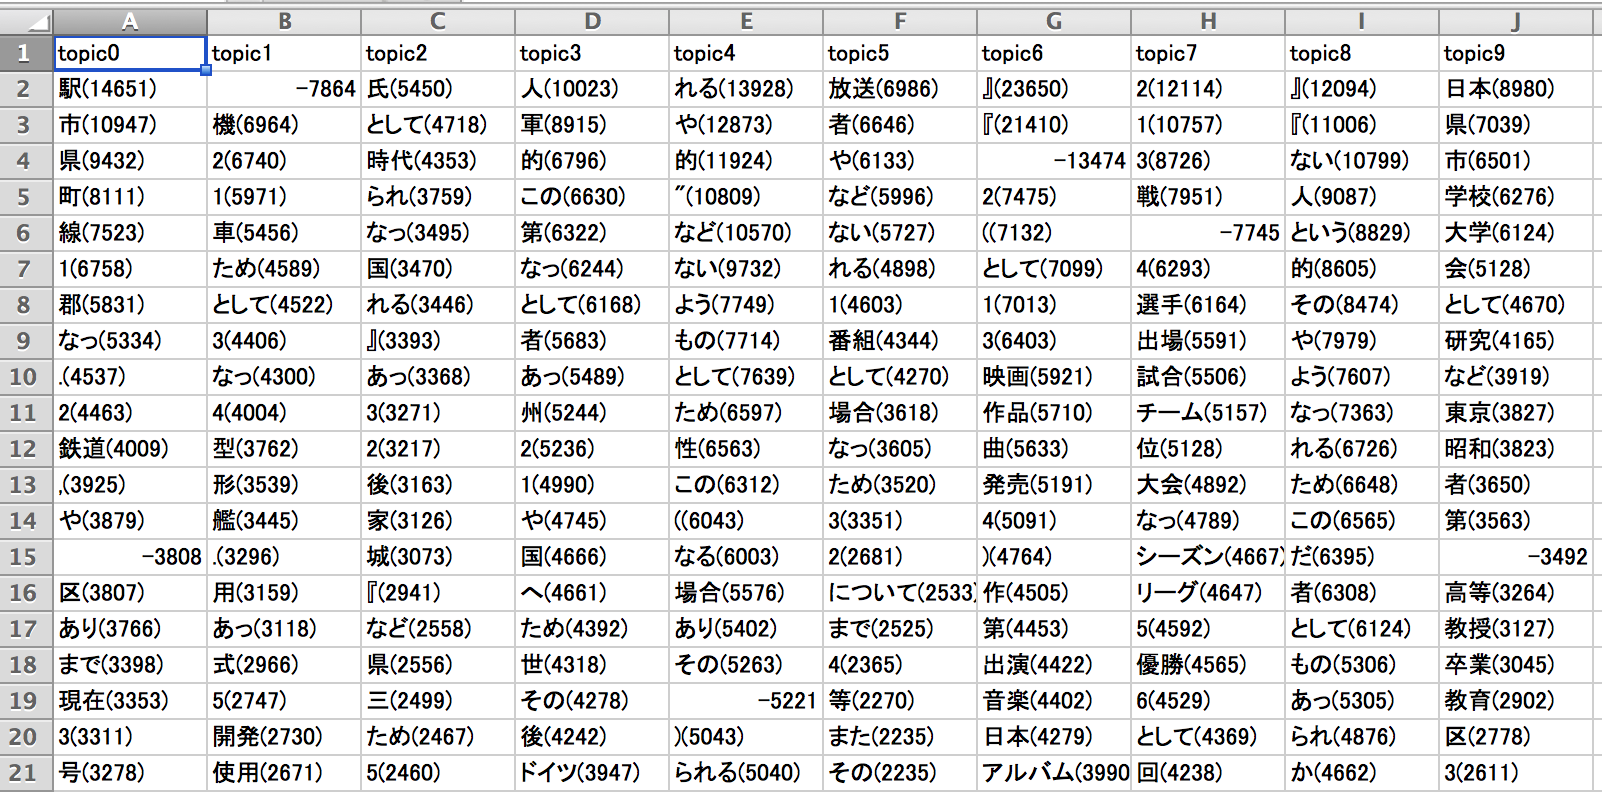
\includegraphics[width=16cm]{topicsoldnoncool.png}
\caption{従来のlda.py}
\end{figure}

\begin{figure}[htb]
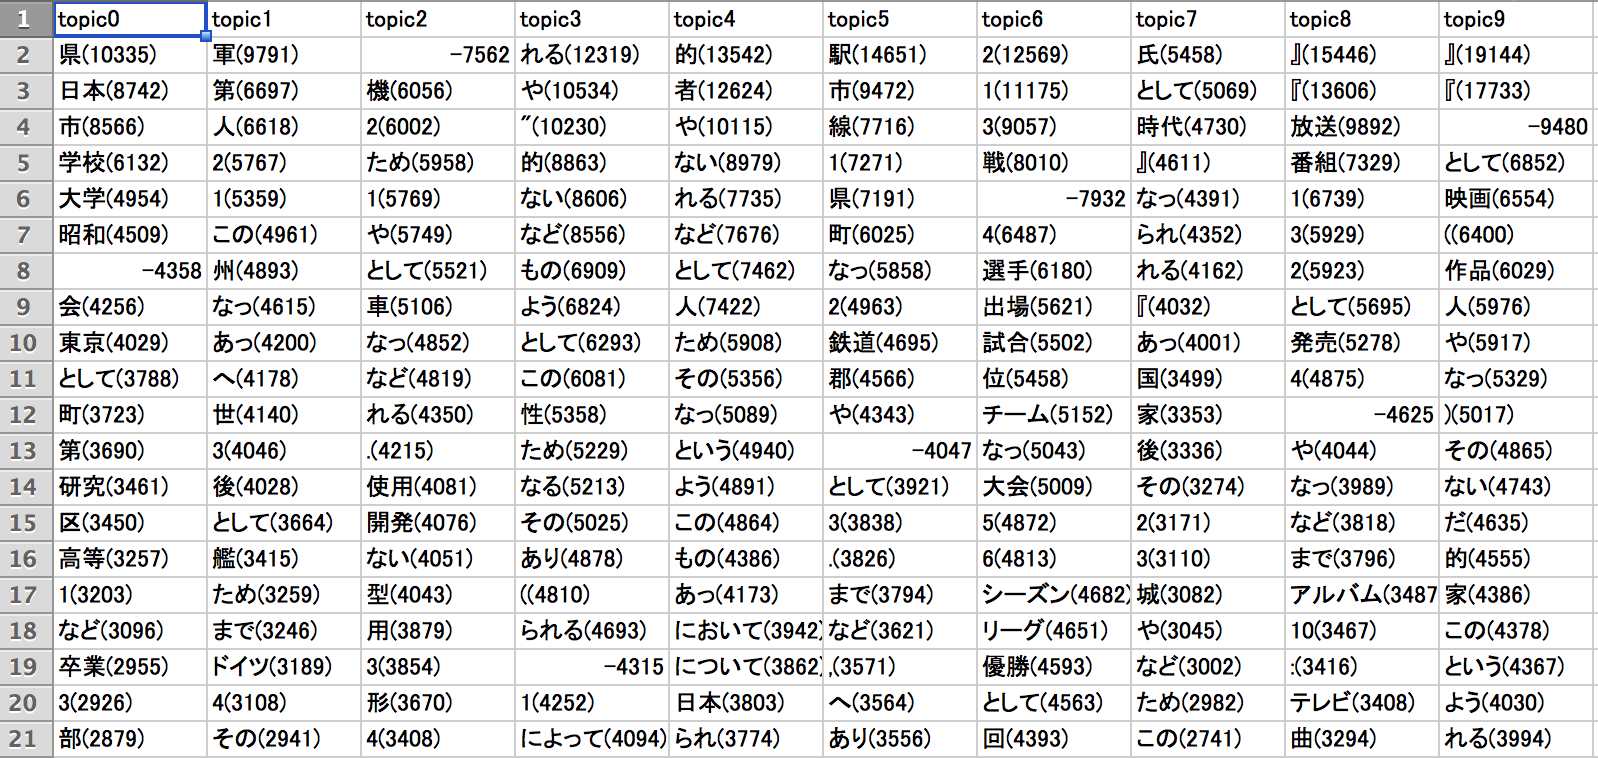
\includegraphics[width=16cm]{topicsnewnoncool.png}
\caption{木村のlda.py}
\end{figure}

\begin{figure}[htb]
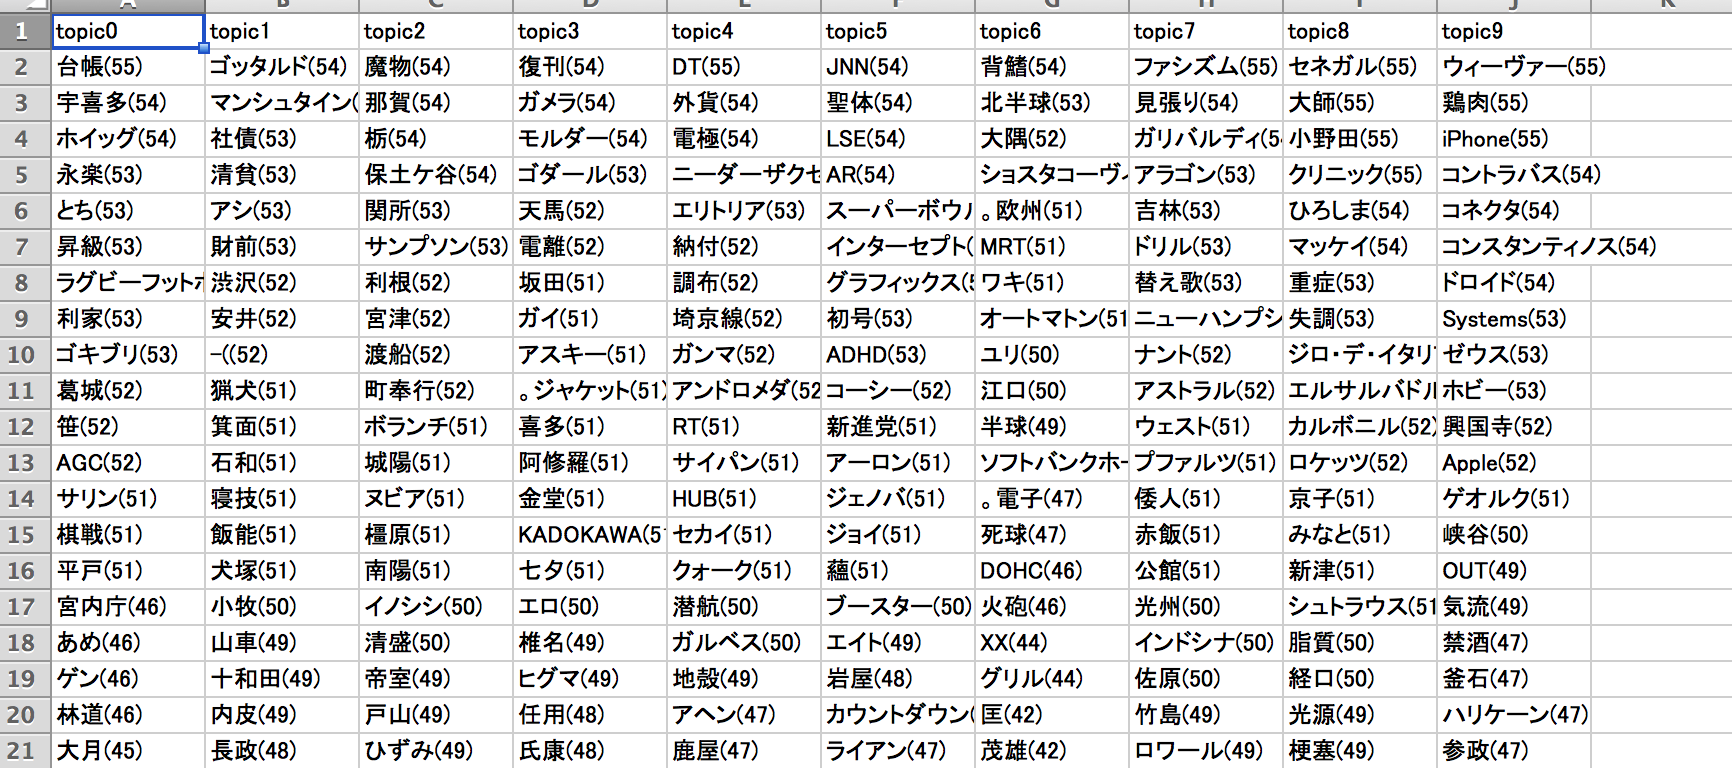
\includegraphics[width=16cm]{topicsoldcool.png}
\caption{従来のlda.py(coolcutter.py済み)}
\end{figure}

\begin{figure}[htb]
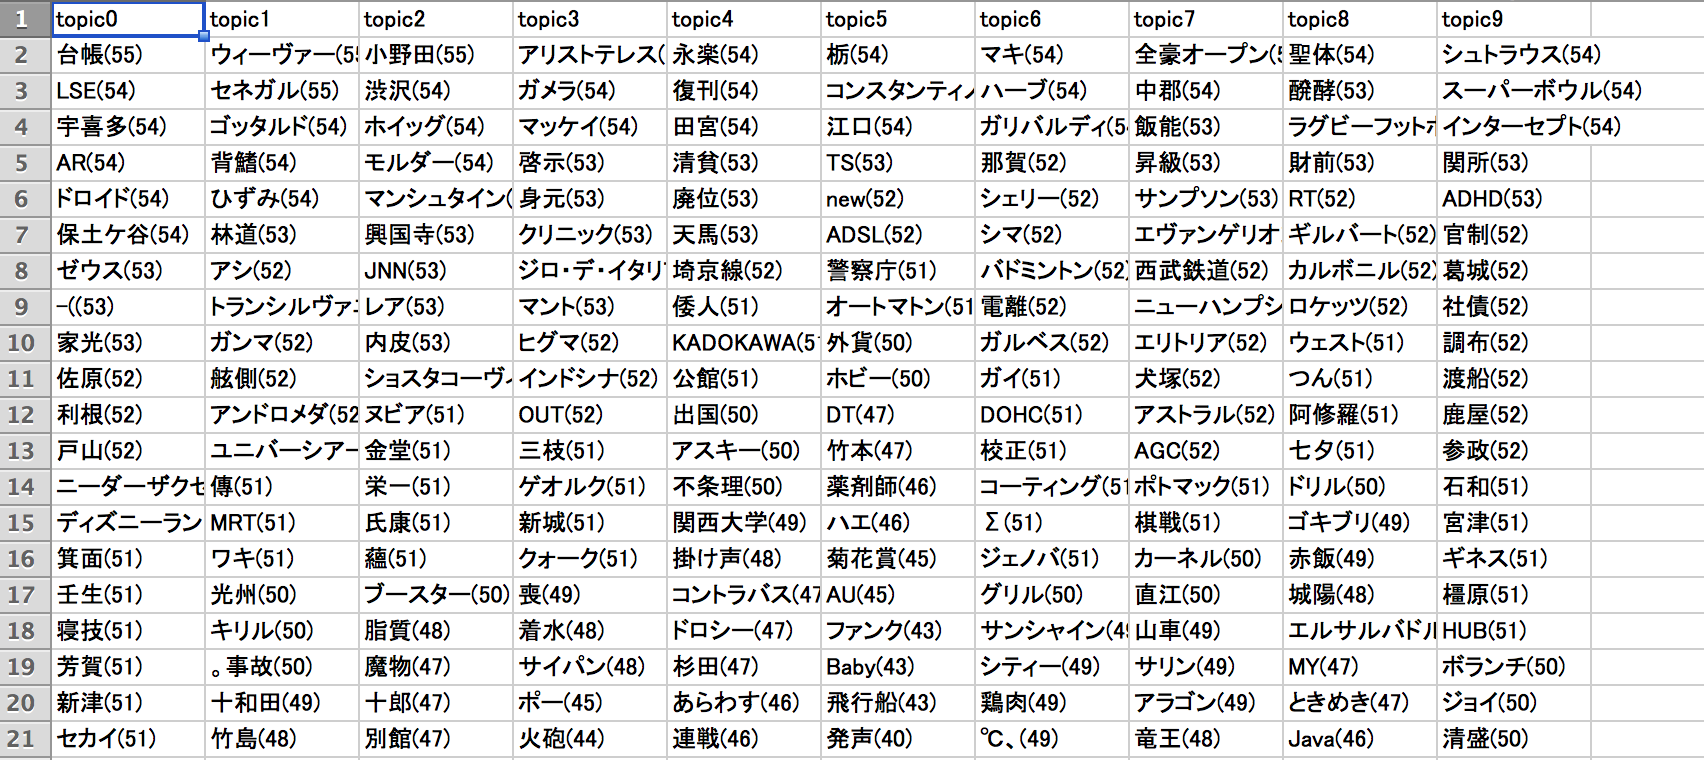
\includegraphics[width=16cm]{topicsnewcool.png}
\caption{木村のlda.py(coolcutter.py済み)}
\end{figure}

\begin{thebibliography}{99}
  \bibitem{murphy} Kevin P. Murphy: Machine Learning: A Probabilistic Perspective (Adaptive Computation and Machine Learning series) The MIT Press, 2012.
  \bibitem{blei} Blei, David M. and Ng, Andrew Y. and Jordan, Michael I.: Latent Dirichlet Allocation,
J. Mach. Learn. Res. 3/1, volume 3, 2003.
\end{thebibliography}
\end{document}
